\documentclass{standalone}
\usepackage{tikz}
\definecolor{cdfdfdf}{RGB}{223,223,223}
\definecolor{cffffff}{RGB}{255,255,255}

\begin{document}
\usetikzlibrary{arrows.meta}

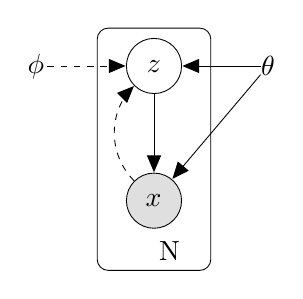
\begin{tikzpicture}[y=0.80pt, x=0.80pt, yscale=-1.000000, xscale=1.000000, inner sep=0pt, outer sep=0pt]
\begin{scope}[cm={{1.25,0.0,0.0,-1.25,(0.0,1052.3622)}}]
  \begin{scope}[shift={(306.491,697.587)}]
    \path[draw=black,fill=cdfdfdf,line join=miter,line cap=butt,miter
      limit=10.00,nonzero rule,line width=0.319pt] (9.9628,0.0000) .. controls
      (9.9628,5.5023) and (5.5023,9.9628) .. (0.0000,9.9628) .. controls
      (-5.5023,9.9628) and (-9.9628,5.5023) .. (-9.9628,0.0000) .. controls
      (-9.9628,-5.5023) and (-5.5024,-9.9628) .. (0.0000,-9.9628) .. controls
      (5.5023,-9.9628) and (9.9628,-5.5024) .. (9.9628,0.0000) -- cycle;
  \end{scope}
    \path[cm={{1.0,0.0,0.0,-1.0,(303.468,695.373)}},fill=black,nonzero rule]
      (0.0000,0.0000) node[above right] (text4171) {$x$};
  \begin{scope}[shift={(306.491,697.587)}]
    \path[draw=black,fill=cffffff,line join=miter,line cap=butt,miter
      limit=10.00,nonzero rule,line width=0.319pt] (9.9628,48.6708) .. controls
      (9.9628,54.1732) and (5.5024,58.6336) .. (0.0000,58.6336) .. controls
      (-5.5023,58.6336) and (-9.9628,54.1732) .. (-9.9628,48.6708) .. controls
      (-9.9628,43.1685) and (-5.5024,38.7081) .. (0.0000,38.7081) .. controls
      (5.5023,38.7081) and (9.9628,43.1685) .. (9.9628,48.6708) -- cycle;
  \end{scope}
    \path[cm={{1.0,0.0,0.0,-1.0,(303.945,744.043)}},fill=black,nonzero rule]
      (0.0000,0.0000) node[above right] (text4181) {$z$};
    \path[cm={{1.0,0.0,0.0,-1.0,(260.848,741.767)}},fill=black,nonzero rule]
      (0.0000,0.0000) node[above right] (text4187) {$\phi$};
    \path[cm={{1.0,0.0,0.0,-1.0,(345.199,742.798)}},fill=black,nonzero rule]
      (0.0000,0.0000) node[above right] (text4193) {$\theta$};
  \begin{scope}[shift={(306.491,697.587)}]
    \path[draw=black,dash pattern=on 2.39pt off 2.39pt,line join=miter,line
      cap=butt,miter limit=10.00,line width=0.319pt] (-38.5088,48.6708) --
      (-10.9710,48.6708);
  \end{scope}
  \begin{scope}[shift={(295.52,746.258)}]
    \path[draw=black,fill=black,line join=miter,line cap=butt,miter
      limit=10.00,nonzero rule,line width=0.319pt] (-5.2035,2.3356) --
      (0.2989,0.0000) -- (-5.2035,-2.3356) -- (-5.2035,2.3356) -- cycle;
  \end{scope}
  \begin{scope}[shift={(306.491,697.587)}]
    \path[draw=black,line join=miter,line cap=butt,miter limit=10.00,line
      width=0.319pt] (38.5088,48.6708) -- (10.9710,48.6708);
  \end{scope}
  \begin{scope}[cm={{-1.0,0.0,0.0,-1.0,(317.462,746.258)}}]
    \path[draw=black,fill=black,line join=miter,line cap=butt,miter
      limit=10.00,nonzero rule,line width=0.319pt] (-5.2035,2.3356) --
      (0.2989,0.0000) -- (-5.2035,-2.3356) -- (-5.2035,2.3356) -- cycle;
  \end{scope}
  \begin{scope}[shift={(306.491,697.587)}]
    \path[draw=black,line join=miter,line cap=butt,miter limit=10.00,line
      width=0.319pt] (38.5088,45.5084) -- (7.1087,8.4005);
  \end{scope}
  \begin{scope}[cm={{-0.64792,-0.7657,0.7657,-0.64792,(313.6,705.988)}}]
    \path[draw=black,fill=black,line join=miter,line cap=butt,miter
      limit=10.00,nonzero rule,line width=0.319pt] (-5.2035,2.3356) --
      (0.2989,0.0000) -- (-5.2035,-2.3356) -- (-5.2035,2.3356) -- cycle;
  \end{scope}
  \begin{scope}[shift={(306.491,697.587)}]
    \path[draw=black,dash pattern=on 2.39pt off 2.39pt,line join=miter,line
      cap=butt,miter limit=10.00,line width=0.319pt] (-7.1856,7.1856) .. controls
      (-16.6444,16.6438) and (-16.6444,32.0271) .. (-7.7582,40.9132);
  \end{scope}
  \begin{scope}[cm={{0.7071,0.7071,-0.7071,0.7071,(298.733,738.5)}}]
    \path[draw=black,fill=black,line join=miter,line cap=butt,miter
      limit=10.00,nonzero rule,line width=0.319pt] (-5.2035,2.3356) --
      (0.2989,0.0000) -- (-5.2035,-2.3356) -- (-5.2035,2.3356) -- cycle;
  \end{scope}
  \begin{scope}[shift={(306.491,697.587)}]
    \path[draw=black,line join=miter,line cap=butt,miter limit=10.00,line
      width=0.319pt] (0.0000,38.5088) -- (0.0000,10.9710);
  \end{scope}
  \begin{scope}[cm={{0.0,-1.0,1.0,0.0,(306.491,708.558)}}]
    \path[draw=black,fill=black,line join=miter,line cap=butt,miter
      limit=10.00,nonzero rule,line width=0.319pt] (-5.2035,2.3356) --
      (0.2989,0.0000) -- (-5.2035,-2.3356) -- (-5.2035,2.3356) -- cycle;
  \end{scope}
    \path[cm={{1.0,0.0,0.0,-1.0,(308.318,675.918)}},fill=black,nonzero rule]
      (0.0000,0.0000) node[above right] (text4239) {N};
  \begin{scope}[shift={(306.491,697.587)}]
    \path[draw=black,line join=miter,line cap=butt,miter limit=10.00,line
      width=0.319pt] (16.5376,62.3527) -- (-16.5376,62.3527) .. controls
      (-18.7386,62.3527) and (-20.5228,60.5685) .. (-20.5228,58.3676) --
      (-20.5228,-21.2037) .. controls (-20.5228,-23.4046) and (-18.7386,-25.1888) ..
      (-16.5376,-25.1888) -- (16.5376,-25.1888) .. controls (18.7386,-25.1888) and
      (20.5228,-23.4046) .. (20.5228,-21.2037) -- (20.5228,58.3676) .. controls
      (20.5228,60.5685) and (18.7386,62.3527) .. (16.5376,62.3527) -- cycle;
  \end{scope}
\end{scope}

\end{tikzpicture}
\end{document}
